\section{Resultados} \label{sec:resultados}

A Tabela~\ref{tab:estudos} reúne os \nTotal\ estudos selecionados. Campos
multirrótulo somam acima de 100\%, e casos sem informação ou não aplicáveis
trazem seus denominadores explícitos.

\begin{table}[tbp]
\centering
\caption{Síntese dos \nTotal\ estudos incluídos (ordem de \texttt{row\_id}). QA: A=Alta, M=Média, B=Baixa; *Val. ext. declarada sem teste externo independente.}
\label{tab:estudos}
{\tiny
\setlength{\tabcolsep}{2.0pt}
\renewcommand{\arraystretch}{0.84}
\begin{tabular*}{0.98\textwidth}{@{}r@{\extracolsep{\fill}} >{\raggedright\arraybackslash}p{3.45cm} c >{\raggedright\arraybackslash}p{2.35cm} l l >{\raggedright\arraybackslash}p{2.95cm} l r@{}}
\toprule
\textbf{ID} & \textbf{Estudo} & \textbf{Ano} & \textbf{Veículo/Tipo} & \textbf{Contrib.} & \textbf{Papel} & \textbf{Cenários} & \textbf{Vaz.} & \textbf{QA} \\
\midrule
2 & \cite{djemaa_quantifying_2026} & 2026 & Prep. (Research Square) & Comparat. & Princ. & 3-cl, Outro & Baixo & 80\%(A) \\
13 & \cite{mohtavipour_deep_2026} & 2026 & Prep. (medRxiv) & Novo mod. & Princ. & PD$\times$HC & Mod. & 90\%(A) \\
21 & \cite{sridhar_early_2026} & 2026 & ICONICA (Anais) & Novo mod. & Princ. & PD$\times$DD, PD$\times$HC & Baixo & 60\%(M) \\
23 & \cite{zannat_label-efficient_2026} & 2026 & Prep. (arXiv) & Novo mod. & Princ. & 3-cl, PD$\times$DD, PD$\times$HC & Alto & 70\%(M) \\
32 & \cite{huang_self-supervised_2025} & 2025 & INDIN (Anais) & Novo mod. & Princ. & Outro, PD$\times$DD, PD$\times$HC & Mod. & 60\%(M) \\
40 & \cite{zhang_generative_2025} & 2025 & Cogn. Comput. & Novo mod. & Princ. & PD$\times$DD, PD$\times$HC & Baixo & 80\%(A) \\
44 & \cite{gao_coverage-aware_2026} & 2026 & Prep. (arXiv) & Novo mod. & Supl. & PD$\times$HC & Baixo & 70\%(M) \\
47 & \cite{abioye_improving_2025} & 2025 & IT J. Res. Dev. & Novo mod. & Val. ext.* & 3-cl & Alto & 30\%(B) \\
49 & \cite{abola_differentiating_2025} & 2025 & Brain Sci. Adv. & Estatíst. & Princ. & Outro & N/A & 83\%(A) \\
51 & \cite{xu_adaptive_2024} & 2024 & BIBM (Anais) & Novo mod. & Princ. & PD$\times$DD & Mod. & 80\%(A) \\
54 & \cite{ren_baseline_2026} & 2026 & Front. Artif. Intell. & Estatíst. & Supl. & -- & N/A & 0\%(B) \\
70 & \cite{varghese_machine_2024} & 2024 & npj Parkinsons Dis. & Base/ML & Princ. & PD$\times$DD, PD$\times$HC & Baixo & 90\%(A) \\
76 & \cite{xing_asa-dsnet_2025} & 2025 & BIBM (Anais) & Novo mod. & Princ. & 3-cl, PD$\times$DD, PD$\times$HC & Indet. & 30\%(B) \\
77 & \cite{pathirathna_neurolens_2026} & 2026 & I2CACIS (Anais) & Plataf. & Princ. & PD$\times$HC & Mod. & 60\%(M) \\
79 & \cite{zeebaree_three-class_2027} & 2026 & Biomed. Signal P. C. & Comparat. & Princ. & 3-cl, Outro, PD$\times$DD & Baixo & 90\%(A) \\
80 & \cite{zhao_multi-scale_2025} & 2025 & BIBM (Anais) & Novo mod. & Princ. & PD$\times$DD & Mod. & 60\%(M) \\
81 & \cite{vasisht_energy_2026} & 2026 & ICMLT (Anais) & Novo mod. & Princ. & PD$\times$HC & Mod. & 50\%(M) \\
83 & \cite{kalathoti_blockchain-enabled_2026} & 2026 & Egypt. Inform. J. & Novo mod. & Princ. & Outro & Mod. & 50\%(M) \\
85 & \cite{suk-ieam_smartwatch-based_2025} & 2025 & i-CREATe (Anais) & Comparat. & Princ. & PD$\times$HC & Indet. & 50\%(M) \\
87 & \cite{wang_parkinsons_2025} & 2025 & IEEE IoT J. & Novo mod. & Princ. & PD$\times$HC & Alto & 60\%(M) \\
89 & \cite{ouabd_parkinsons_2026} & 2026 & IRASET (Anais) & Comparat. & Princ. & PD$\times$DD, PD$\times$HC & Baixo & 70\%(M) \\
90 & \cite{vu_simple_2026} & 2026 & VFAST Trans. SE & Novo mod. & Princ. & PD$\times$DD, PD$\times$HC & Baixo & 70\%(M) \\
92 & \cite{yu_improved_2024} & 2024 & Electronics & Novo mod. & Princ. & 3-cl, PD$\times$DD, PD$\times$HC & Alto & 60\%(M) \\
99 & \cite{win_checkpd_2026} & 2026 & Prep. (JMIR Preprints) & Comparat. & Supl. & PD$\times$HC & Baixo & 80\%(A) \\
101 & \cite{wei_sgc-rml_2026} & 2026 & Prep. (arXiv) & Novo mod. & Princ. & 3-cl & Baixo & 90\%(A) \\
104 & \cite{haque_eco-xpd_2026} & 2026 & Inf. Fusion & Novo mod. & Princ. & PD$\times$HC & Mod. & 60\%(M) \\
105 & \cite{padilha_identificacao_2025} & 2025 & ERI-GO (Anais) & Comparat. & Princ. & DD$\times$HC, PD$\times$DD, PD$\times$HC & Mod. & 70\%(M) \\
108 & \cite{padilha_parkinsons_2024} & 2024 & ERI-GO (Anais) & Comparat. & Princ. & PD$\times$DD, PD$\times$HC & Mod. & 70\%(M) \\
109 & \cite{lobo_parkinsons_2025} & 2025 & ERI-GO (Anais) & Comparat. & Princ. & DD$\times$HC, PD$\times$DD, PD$\times$HC & Mod. & 60\%(M) \\
\bottomrule
\end{tabular*}
}
\end{table}


\subsection{Panorama, Veículos e Contribuições (QP1)}

A adoção do PADS cresceu rápido: \nAnoDoisQuatro\ estudos em 2024, \nAnoDoisCinco\
em 2025 e \nAnoDoisSeis\ em 2026 (\pctAnoDoisSeis, Figura~\ref{fig:ano_contrib},
onde~\cite{zeebaree_three-class_2027} consta em 2027 no Zotero, mas tem DOI de
2026). Predominam anais (\nAnais/\nTotal) e periódicos (\nPeriodicos/\nTotal),
além de \nPreprints\ \textit{preprints} (\nPreArxiv\ arXiv, \nPreMedrxiv\
medRxiv, \nPreRS\ Research Square e \nPreJMIR\ JMIR Preprints).

Mais da metade propõe novos modelos (\nContribNovoModelo/\nTotal,
\pctContribNovoModelo), seguidos por \nContribComparativo\ estudos comparativos,
\nContribEstatistica\ estatísticos, \nContribPlataforma\ plataforma e o
artigo-base (categoria Outro na Figura~\ref{fig:ano_contrib}). O PADS é fonte
principal em \nPapelPrincipal/\nTotal\ (\pctPapelPrincipal) trabalhos,
suplementar em \nPapelSuplementar\ e declarado como validação externa
em~\cite{abioye_improving_2025}, enquanto \nMultiBase\ combinam outras bases
(\nOutroPublico\ públicas e \nPrivadoProprio\ privadas, com \nMultiBaseSobrep\
sobreposições).

\begin{figure}[htb]
\centering
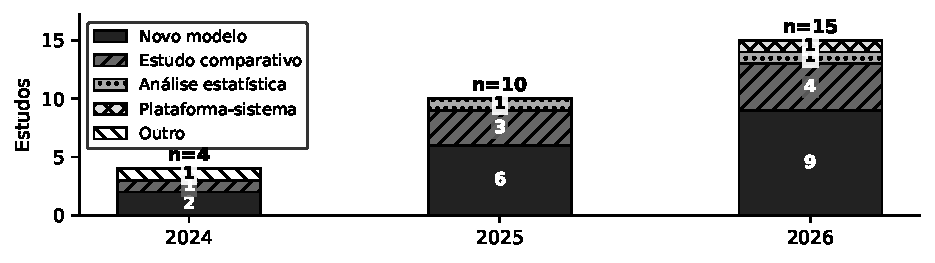
\includegraphics[width=0.78\textwidth]{figuras/fig2_ano_contribuicao.pdf}
\caption{Distribuição dos \nTotal\ estudos por ano e tipo de contribuição.}
\label{fig:ano_contrib}
\end{figure}

\subsection{Tarefas de Classificação e Recortes do Dataset (QP2)}

Pela Tabela~\ref{tab:recorte}, quase toda a literatura usa séries inerciais
(\nModIMU/\nTotal), combinando giroscópio e acelerômetro. O PDNMS e metadados
entram como apoio, salvo dois estudos restritos ao
questionário~\cite{ouabd_parkinsons_2026,padilha_parkinsons_2024}. Entre os
\nModIMU\ trabalhos com IMU, \nTarIMUTodas/\nModIMU\ usam todas as 11 tarefas
motoras, \nTarIMUSubconj/\nModIMU\ apenas um subconjunto e \nPunhoIMUAmbos/\nModIMU\
ambos os punhos, havendo omissões de relato (\nTarIMUNaoRep/\nModIMU\ sem
detalhar tarefas, \nPunhoIMUNaoRep/\nModIMU\ sem especificar punho e
\nSensIMUVazio/\nModIMU\ sem informar sensores~\cite{xing_asa-dsnet_2025}, além de
``IMU de 6 canais'' na categoria Outro~\cite{wei_sgc-rml_2026}, sendo os outros
dois registros sem campo de sensores os estudos sem IMU).

O $N$ amostral consta em \nPartRep/\nTotal\ artigos (\nPartMin--\nPartMax\
participantes, mediana \nPartMediana). Frente ao PADS oficial (276~PD, 79~HC,
114~DD), há divergências em~\cite{djemaa_quantifying_2026} (295/71/103),
\cite{zannat_label-efficient_2026} (291/79/99) e~\cite{vu_simple_2026} (HC=114 e
DD=79 invertidos). Domina PD$\times$HC (\nCenPDHC/\nTotal, \pctCenPDHC),
enquanto PD$\times$DD (\nCenPDDD/\nTotal), 3 classes (classificação simultânea
PD, DD e HC, \nCenTresClasses/\nTotal), DD contra HC (DD$\times$HC,
\nCenDDHC/\nTotal) e outros recortes (Outro, \nCenOutro/\nTotal) aparecem menos.

\begin{table}[htbp]
\centering
\caption{Recorte do dataset PADS nos \nTotal\ estudos (QP2). *Campos multirrótulo (somas acima de 100\%); contagens na ordem das categorias.}
\label{tab:recorte}
{\scriptsize
\setlength{\tabcolsep}{3.5pt}
\begin{tabular}{@{}l l l r@{}}
\toprule
\textbf{Dimensão} & \textbf{Categorias (na ordem das contagens)} & \textbf{Contagens ($n$)} & \textbf{Base} \\
\midrule
Modalidade* & Série temporal (IMU) / Questionário (PDNMS) / Metadados & 27; 9; 8 & $N=29$ \\
Tarefas motoras & Todas / Subconjunto / Não rep. / N/A & 14; 7; 6; 2 & $N=29$ \\
Sensores* & Giroscópio / Acelerômetro / Outro / Não rep. ou N/A & 25; 24; 1; 3 & $N=29$ \\
Punho(s) & Ambos / Não rep. / Esq. ou Dir. (1 cada) / N/A & 16; 9; 2; 2 & $N=29$ \\
Cenários* & PD$\times$HC / PD$\times$DD / 3 classes / Outro / DD$\times$HC / N/A & 20; 15; 7; 5; 2; 1 & $N=29$ \\
\bottomrule
\end{tabular}
}
\end{table}


\subsection{Pré-processamento, Atributos e Modelos (QP3)}

Na entrada dos modelos, predominam séries temporais (categoria ``Série bruta''
do formulário, \nRepBruta/\nTotal, \pctRepBruta) sobre atributos manuais
(\nRepHandcrafted/\nTotal), além do uso pontual de tempo-frequência e
BOSS/\textit{embeddings} (\nRepTF/\nTotal\ cada). Como a categoria ``Série bruta''
reuniu sinais puros e pré-processados, a análise dos \nModIMU\ estudos com IMU
mostra preparos muito distintos: oito removem o transiente vibratório inicial, em regra de 0,5~s como
no artigo-base~\cite{varghese_machine_2024} (e 1~s em um caso). Na filtragem,
cinco corrigem a gravidade por $\ell_1$-\textit{trend filtering} ou pelo
\textit{script} oficial~\cite{padilha_identificacao_2025}, quatro aplicam
filtros passa-faixa ou Butterworth até 20~Hz~\cite{win_checkpd_2026}, dois
decompõem sub-bandas na própria rede e dois declaram não filtrar, havendo ainda
casos pontuais de subtração da média e suavização. Só três reamostram a taxa de
100~Hz (para 64, 40 ou 20~Hz). Quanto à segmentação, cinco dividem séries
longas em blocos de 1.024 pontos e 13 trabalham com sub-janelas curtas
(1--4~s ou 20--512 amostras), por vezes sobrepostas~\cite{gao_coverage-aware_2026}.
Na escala, 12 relatam padronização \textit{z-score} ou por canal (sete restrita
ao treino ou ao sujeito~\cite{djemaa_quantifying_2026} e cinco sem explicitar o
escopo), dois citam normalização genérica e os demais omitem a etapa.

Na modelagem (Figura~\ref{fig:cen_fam}), a família DL lidera (\nFamDL/\nTotal,
\pctFamDL), seguido de ML clássico (\nFamML/\nTotal),
híbridos/\textit{ensemble} (\nFamHybrid), generativos (\nFamGen) e
auto-supervisionados (SSL, \nFamSSL), com foco em PD$\times$HC. No
desbalanceamento, \nBalNenhum/\nTotal\ não aplicam correção, e o restante usa
perturbações ou ponderação (\nBalOutro), SMOTE (\nBalSMOTE) e GANs (\nBalGAN),
com \nBalNaoRep\ sem relato e \nBalNA\ N/A.

\begin{figure}[htb]
\centering
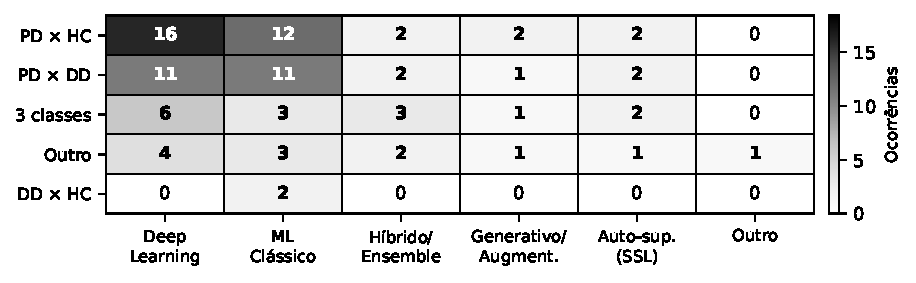
\includegraphics[width=0.78\textwidth]{figuras/fig3_cenario_familia.pdf}
\caption{Cenários de classificação vs.\ famílias de algoritmos ($N=\nTotal$).}
\label{fig:cen_fam}
\end{figure}

\subsection{Validação, Métricas, Vazamento e Desempenho (QP4)}

Pela Tabela~\ref{tab:validacao}, \textit{k-fold} (validação cruzada em $k$ dobras,
\nValKfold/\nTotal) predomina, com \textit{hold-out} (partição fixa treino/teste,
\nValHoldout), enquanto CV aninhada (\nValAninhada) e LOSO
(\textit{leave-one-subject-out}, \nValLOSO~\cite{sridhar_early_2026}) são raras.
Embora \nUnidPart/\nAplicaveisVaz\ (\pctUnidPart) preditivos dividam por
participante (6 inferidos, 5 sem relato), a Figura~\ref{fig:risco_vaz} mostra
que só \nRiscoBaixo/\nAplicaveisVaz\ (\pctRiscoBaixoAplic) mantêm risco baixo de
vazamento (Seção~\ref{sec:desvio_qa}). Outros \nRiscoModerado\ têm risco de
vazamento moderado (pré-processamento omitido) e \nRiscoAlto, alto, por
balanceamento ou janelamento pré-\textit{split}~%
\cite{zannat_label-efficient_2026,abioye_improving_2025,wang_parkinsons_2025,yu_improved_2024}.

\begin{table}[htbp]
\centering
\caption{Protocolos de validação e risco de vazamento reportado (QP4). *Multirrótulo; $N=27$ exclui \nNaoAplicaveisVaz\ análises estatísticas (N/A).}
\label{tab:validacao}
{\scriptsize
\setlength{\tabcolsep}{3.2pt}
\begin{tabular}{@{}l l l r@{}}
\toprule
\textbf{Aspecto} & \textbf{Categorias (na ordem das contagens)} & \textbf{Contagens ($n$)} & \textbf{Denominador} \\
\midrule
Estratégia* & k-fold CV / Hold-out / CV aninhada / Não rep. / LOSO / Outra & 24; 9; 6; 3; 1; 1 & $N=29$ \\
Unid. particionamento & Participante / Não reportado / Não se aplica & 22 (81,5\%); 5; 2 & $N=27$ (+2 N/A) \\
Separação participante & Sim explícita / Sim inferida / Pouco claro / N/A & 16; 6; 5; 2 & $N=27$ (+2 N/A) \\
Momento balanceam. & Só no treino / Antes do split / Não rep. / N/A & 11; 4; 2; 12 & $N=29$ \\
Pré-proc. só no treino & Sim / Não / Não reportado / Não se aplica & 10; 4; 13; 2 & $N=27$ (+2 N/A) \\
Risco de vazamento & Baixo / Moderado / Alto / Indeterminado / N/A & 10; 11; 4; 2; 2 & $N=27$ (+2 N/A) \\
\bottomrule
\end{tabular}
}
\end{table}


Nenhum estudo fez validação externa entre bases (\nValExtSim/\nTotal): embora
\nMultiBase\ combinem bases e~\cite{abioye_improving_2025} cite o PADS para
generalização, todos retreinaram internamente. Nas métricas, F1
(\nMetFOne/\nTotal) e acurácia (\nMetAcc/\nTotal) superam Bal.\ Acc.\
(\nMetBalAcc/\nTotal) e AUC (\nMetAUC/\nTotal). A Tabela~\ref{tab:desempenho}
lista o melhor resultado por \texttt{row\_id}, sem comparação direta.

\begin{figure}[htb]
\centering
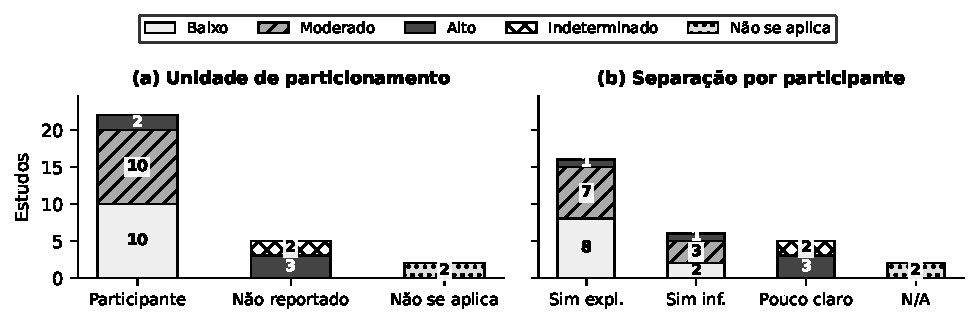
\includegraphics[width=0.78\textwidth]{figuras/fig4_risco_vazamento.pdf}
\caption{Risco de vazamento por unidade (a) e separação por sujeito (b).}
\label{fig:risco_vaz}
\end{figure}

\begin{table}[htbp]
\centering
\caption{Melhor resultado (\texttt{row\_id}, sem ranqueamento). HO = \textit{hold-out}, Anin.\ = CV aninhada, LOTO = \textit{leave-one-task-out}, Vaz.\ = risco de vazamento.}
\label{tab:desempenho}
{\tiny
\setlength{\tabcolsep}{1.4pt}
\renewcommand{\arraystretch}{0.68}
\begin{tabular*}{0.99\textwidth}{@{}r@{\extracolsep{\fill}} >{\raggedright\arraybackslash}p{3.10cm} >{\raggedright\arraybackslash}p{2.12cm} >{\raggedright\arraybackslash}p{2.52cm} >{\raggedright\arraybackslash}p{1.12cm} >{\raggedright\arraybackslash}p{2.36cm} l@{}}
\toprule
\textbf{ID} & \textbf{Estudo} & \textbf{Cenário} & \textbf{Modelo/Método} & \textbf{Métrica} & \textbf{Resultado} & \textbf{Validação (Vaz.)} \\
\midrule
2 & \cite{djemaa_quantifying_2026} & Outro (PD vs. non-PD) & BTE+SMOTE+RF & AUC & 0,842 $\pm$ 0,043 & k-fold (Baixo) \\
13 & \cite{mohtavipour_deep_2026} & PD$\times$HC & Multi-stream CNN-Transf. & Bal. Acc. & 85,89\% $\pm$ 3,93\% & k-fold (Mod.) \\
21 & \cite{sridhar_early_2026} & PD$\times$HC & CNN-BiLSTM + Attention & Accuracy & 95,30\% $\pm$ 1,10\% (10-fold) & Anin.+LOSO+k-fold (Baixo) \\
23 & \cite{zannat_label-efficient_2026} & PD$\times$HC & Interleaved self-attn (ours) & AUROC & 0,963 & LOTO+k-fold (Alto) \\
32 & \cite{huang_self-supervised_2025} & Outro (PL vs. PD) & Ours & Acc/F1/AUC & 81,00\% / 0,81 / 0,81 & HO (Mod.) \\
40 & \cite{zhang_generative_2025} & PD$\times$HC & BOSS+SVM (TremorGANs) & Accuracy & 87,60\% $\pm$ 1,40\% & k-fold (Baixo) \\
44 & \cite{gao_coverage-aware_2026} & PD$\times$HC & RBF-SVM (Ours) & Bal. Acc. & 80,52\% $\pm$ 9,08\% & Anin.+k-fold (Baixo) \\
47 & \cite{abioye_improving_2025} & 3 classes & Stacking (CatBoost+RF+LR) & Accuracy & 100,00\% & HO+k-fold (Alto) \\
49 & \cite{abola_differentiating_2025} & Outro (6 grupos) & Reg. Logística Multinom. & Pseudo R$^2$ & 0,068 (LR $\chi$$^2$=1740, p<0,001) & Não rep. (N/A) \\
51 & \cite{xu_adaptive_2024} & PD$\times$DD (StretchHold) & ADAMIL (Ours) & Accuracy & 81,44\% & k-fold (Mod.) \\
54 & \cite{ren_baseline_2026} & N/A (Correl.) & Correl. de Spearman & Spearman r & r = -0,171 (p=0,0071) & Não rep. (N/A) \\
70 & \cite{varghese_machine_2024} & PD$\times$HC & Stacking (IMU+PDNMS) & Bal. Acc. & 91,16\% (4,92\%) & Anin.+k-fold (Baixo) \\
76 & \cite{xing_asa-dsnet_2025} & 3 classes & ASA-DSNet & Accuracy & 80,85\% & Anin.+k-fold (Indet.) \\
77 & \cite{pathirathna_neurolens_2026} & PD$\times$HC & 1D CNN (8-bit) & Bal. Acc. & 70,20\% & HO+k-fold (Mod.) \\
79 & \cite{zeebaree_three-class_2027} & 3 classes & Soft-voting XGB-LGBM & Accuracy & 72,28\% $\pm$ 3,19\% & HO+k-fold (Baixo) \\
80 & \cite{zhao_multi-scale_2025} & PD$\times$DD (CrossArms) & MFAM & Accuracy & 81,29\% & k-fold (Mod.) \\
81 & \cite{vasisht_energy_2026} & PD$\times$HC & Random Forest & Accuracy & 82,86\% & HO+k-fold (Mod.) \\
83 & \cite{kalathoti_blockchain-enabled_2026} & Outro (PD vs. No PD) & CNN-Transformer & Accuracy & 97,29\% & k-fold (Mod.) \\
85 & \cite{suk-ieam_smartwatch-based_2025} & PD$\times$HC & 1D CNN (Finger-to-Finger) & Accuracy & 87,32\% & Não rep. (Indet.) \\
87 & \cite{wang_parkinsons_2025} & PD$\times$HC & MSF-CANet & Accuracy & 92,39\% & Anin.+k-fold (Alto) \\
89 & \cite{ouabd_parkinsons_2026} & PD$\times$HC & Random Forest & Bal. Acc. & 93,24\% & HO+k-fold (Baixo) \\
90 & \cite{vu_simple_2026} & PD$\times$HC & LR & Bal. Acc. & 79,26\% $\pm$ 5,50\% & Anin.+k-fold (Baixo) \\
92 & \cite{yu_improved_2024} & PD$\times$HC & CA\_LSTM\_FCN (acc + rot) & Accuracy & 92,15\% & k-fold (Alto) \\
99 & \cite{win_checkpd_2026} & PD$\times$HC (Relaxed/Rest) & Conv1D-BiLSTM & ROC AUC & 0,842 & HO+k-fold (Baixo) \\
101 & \cite{wei_sgc-rml_2026} & 3 classes & PatchTST + Quality & AUC & 0,825 & HO+k-fold (Baixo) \\
104 & \cite{haque_eco-xpd_2026} & PD$\times$HC & Eco-xPD (c/ xReDA) & F1-score & 93,60\% $\pm$ 1,03\% & HO (Mod.) \\
105 & \cite{padilha_identificacao_2025} & PD$\times$HC (DP vs. CO) & LightGBM & Accuracy & 84,05\% $\pm$ 3,16\% & k-fold (Mod.) \\
108 & \cite{padilha_parkinsons_2024} & PD$\times$HC & Random Forest & Bal. Acc. & 87,00\% & k-fold (Mod.) \\
109 & \cite{lobo_parkinsons_2025} & DD$\times$HC & Extra Trees & Bal. Acc. & 82,48\% & k-fold (Mod.) \\
\bottomrule
\end{tabular*}
}
\end{table}


\subsection{Qualidade e Reprodutibilidade (QP4)}

Qualidade metodológica média (QA): \qaMediaPct\ (mediana \qaMedianaPct,
\qaMinPct--\qaMaxPct), com \nQAMedia/\nTotal\ na faixa Média, \nQAAlta\ Alta e
\nQABaixa\ Baixa (Seção~\ref{sec:desvio_qa}). Na Figura~\ref{fig:qa}, QA1--QA2
vão bem, mas falham QA4 (parcial: \nQAQuatroPart/\nTotal) e QA5:
\nCodDisponivel/\nTotal\ (\pctCodDisponivel) abrem
código~\cite{mohtavipour_deep_2026,xu_adaptive_2024,wei_sgc-rml_2026} ou
ambos~\cite{varghese_machine_2024}.

\begin{figure}[htb]
\centering
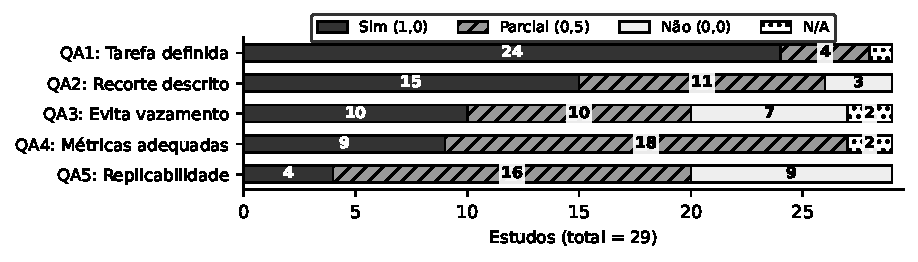
\includegraphics[width=0.78\textwidth]{figuras/fig5_qa.pdf}
\caption{Distribuição das respostas de qualidade (QA1--QA5) nos \nTotal\ estudos.}
\label{fig:qa}
\end{figure}

\subsection{Lacunas Identificadas e Oportunidades (QP5)}

A Tabela~\ref{tab:lacunas} sintetiza cinco lacunas (\nSemLimitacao\ sem limitações
e \nSemLacuna\ sem trabalhos futuros): multimodalidade/explicabilidade
(XAI)/calibração (\nLacunaMultimodalXAI/\nTotal), severidade/vida livre
(\nLacunaLongitSev/\nTotal), coortes externas (\nLacunaValExt/\nTotal) e
diagnóstico diferencial (\nLacunaPDDD/\nTotal), com \pctCodNenhum\ sem
código/dados e \pctCodNaoRep\ sem menção.

\begin{table}[htbp]
\centering
\caption{Síntese temática das limitações reportadas, lacunas e reprodutibilidade nos \nTotal\ estudos (QP5).}
\label{tab:lacunas}
{\scriptsize
\setlength{\tabcolsep}{3pt}
\begin{tabular}{@{}>{\raggedright\arraybackslash}p{3.8cm} r >{\raggedright\arraybackslash}p{4.0cm} >{\raggedright\arraybackslash}p{4.1cm}@{}}
\toprule
\textbf{Tema / Lacuna} & \textbf{$n/N$ (\%)} & \textbf{Exemplos no corpus} & \textbf{Implicação para o PADS} \\
\midrule
Ausência de validação externa / coortes multicêntricas & 15/29 (51,7\%) & \cite{djemaa_quantifying_2026}, \cite{zannat_label-efficient_2026}, \cite{huang_self-supervised_2025} (e outros 12) & Treino/teste restrito ao PADS; validação externa = 0/29. \\
Dificuldade no diagnóstico diferencial (PD$\times$DD) & 11/29 (37,9\%) & \cite{zannat_label-efficient_2026}, \cite{huang_self-supervised_2025}, \cite{zhang_generative_2025} (e outros 8) & Menor acurácia na fronteira PD vs.\ DD/tremor essencial. \\
Falta de severidade clínica (MDS-UPDRS/H\&Y) e vida livre/longitudinal & 17/29 (58,6\%) & \cite{zannat_label-efficient_2026}, \cite{huang_self-supervised_2025}, \cite{abola_differentiating_2025} (e outros 14) & Falta MDS-UPDRS/H\&Y e coleta em vida livre. \\
Falta de multimodalidade, XAI, calibração e justiça demográfica & 20/29 (69,0\%) & \cite{djemaa_quantifying_2026}, \cite{zhang_generative_2025}, \cite{abioye_improving_2025} (e outros 17) & Fusão, explicabilidade clínica, calibração e controle de vazamento. \\
Indisponibilidade de código/dados derivados (reprodutibilidade) & 25/29 (86,2\%) & \cite{djemaa_quantifying_2026}, \cite{zannat_label-efficient_2026}, \cite{huang_self-supervised_2025} (e outros 22) & Compartilhamento de código/dados em apenas \nCodDisponivel/\nTotal. \\
\bottomrule
\end{tabular}
}
\end{table}


\subsection{Literatura Cinzenta: Preprints e Análise de Sensibilidade}
\label{sec:preprints}

Os \nPreprints\ \textit{preprints} (2026, DL, Tabela~\ref{tab:preprints}) focam
PD$\times$HC (só 1 em PD$\times$DD), com QA média maior (\qaMediaPrePct\
vs.\ \qaMediaRevPct) e mais risco baixo de vazamento pelo controle no
\textit{augmentation}~\cite{djemaa_quantifying_2026}, salvo risco alto de
vazamento por janelamento~\cite{zannat_label-efficient_2026}. Sem eles
($n=\nRevisadosPares$), 2026 cai (\pctAnoDoisSeis\ a \pctRevAnoDoisSeis,
\nRevAnoDoisSeis/\nRevisadosPares), risco baixo de vazamento (\pctRiscoBaixoAplic\
a \pctRevRiscoBaixoAplic) e código (\pctCodDisponivel\ a \pctRevCodDisp),
mantendo DL, PD$\times$HC (PD$\times$DD: \pctRevPDDD\ vs.\ \pctCenPDDD) e
\nValExtSim/\nRevisadosPares\ em validação externa.

\begin{table}[htbp]
\centering
\caption{Revisados ($n=23$) vs.\ \textit{preprints} ($n=6$) e sensibilidade total ($n=29$).}
\label{tab:preprints}
{\scriptsize
\setlength{\tabcolsep}{3.5pt}
\renewcommand{\arraystretch}{0.74}
\begin{tabular*}{0.78\textwidth}{@{}l@{\extracolsep{\fill}} r r r@{}}
\toprule
\textbf{Indicador} & \textbf{Revisados ($n=23$)} & \textbf{Preprints ($n=6$)} & \textbf{Total ($n=29$)} \\
\midrule
Publicação em 2026 & 9/23 (39,1\%) & 6/6 (100,0\%) & 15/29 (51,7\%) \\
Contribuição: Novo modelo & 13/23 & 4/6 & 17/29 \\
Cenário PD$\times$DD & 14/23 (60,9\%) & 1/6 (16,7\%) & 15/29 (51,7\%) \\
Família: Deep Learning & 16/23 (69,6\%) & 6/6 (100,0\%) & 22/29 (75,9\%) \\
Separação por participante (Sim) & 16/21 & 6/6 & 22/27 \\
Risco de vazamento Baixo & 6/21 (28,6\%) & 4/6 (66,7\%) & 10/27 (37,0\%) \\
Qualidade QA (faixa Alta) & 5/23 (21,7\%) & 4/6 (66,7\%) & 9/29 (31,0\%) \\
Qualidade QA (média) & 60,6\% & 80,0\% & 64,6\% \\
Código/dados disponíveis & 2/23 & 2/6 & 4/29 \\
\bottomrule
\end{tabular*}
}
\end{table}

